%
% File coling2016.tex
%
% Contact: mutiyama@nict.go.jp
%%
%% Based on the style files for COLING-2014, which were, in turn,
%% Based on the style files for ACL-2014, which were, in turn,
%% Based on the style files for ACL-2013, which were, in turn,
%% Based on the style files for ACL-2012, which were, in turn,
%% based on the style files for ACL-2011, which were, in turn, 
%% based on the style files for ACL-2010, which were, in turn, 
%% based on the style files for ACL-IJCNLP-2009, which were, in turn,
%% based on the style files for EACL-2009 and IJCNLP-2008...

%% Based on the style files for EACL 2006 by 
%%e.agirre@ehu.es or Sergi.Balari@uab.es
%% and that of ACL 08 by Joakim Nivre and Noah Smith

\documentclass[11pt]{article}
\usepackage{coling2016}
\usepackage{times}
\usepackage{url}
\usepackage{latexsym}
\usepackage{graphicx}
\usepackage{amsmath}


%\setlength\titlebox{5cm}

% You can expand the titlebox if you need extra space
% to show all the authors. Please do not make the titlebox
% smaller than 5cm (the original size); we will check this
% in the camera-ready version and ask you to change it back.


\title{Predicting the Tolerance Level of Religious Discourse Through Computational Linguistics}

\author{Nicolas Venuti \\
  Data Science Institute \\
  University of Virginia \\
  Charlottesville, VA USA \\
  {nmv7de@virginia.edu} \\\And
  Hope McIntyre \\
  Data Science Institute \\
  University of Virginia \\
  Charlottesville, VA USA \\
  {hm7zg@virginia.edu}\\\And
  Donald E. Brown \\
  Data Science Institute \\
  University of Virginia \\
  Charlottesville, VA USA \\
  {brown@virginia.edu} \\}

\date{}

\begin{document}
\maketitle
\begin{abstract}
 Religious violence is one of the biggest and most complicated problems facing the world today. The number of incidents has been increasing in recent years and, unfortunately, scalable and accurate systems to predict which groups are likely to engage in such actions are not keeping pace. Additionally, this problem is compounded by lingual and cultural differences, which limit the effectiveness of understanding how tolerant or intolerant a group is without bias. To circumvent this challenge, recent studies indicate promise in the analysis of the performative character of discourse (how words are used) to estimate the tolerance level, rather than using the semantic or emotive character of text (what the words mean or imply). Using expert estimates of linguistic flexibility, a representation of the performative character of text, and thus also predictive of a text’s tolerance level, this paper describes (a) new approaches to automating the quantification of the performative character of words and (b) the predictive efficacy of these approaches versus traditional semantic indicators of tolerance or intolerance. To implement the pipeline, a judgment identifier was developed along with multiple semantic density algorithms to extract the frequency of judgments and flexibility of keyword contexts, respectively. Test results show that text mining algorithms can accurately estimate the language flexibility of religious discourse. These results provide evidence that the performative characteristics of language better predict tolerance level than the semantic characteristics of language.

\end{abstract}

\section{Introduction}\label{Intro}

\blfootnote{
    %
    % 
    %
    \hspace{-0.65cm}  
    This work is licenced under a Creative Commons 
     Attribution 4.0 International License.
     License details:
     \url{http://creativecommons.org/licenses/by/4.0/}
    %
    
}

Religious violence has long been one of the most destructive and divisive acts impacting society and, unfortunately, the number of casualties associated with these acts has been rising in recent years. For example, in 2014 alone, 12,737 deaths could be attributed to the operations of just two separate radical terrorist groups: Boko Haram with 6,664 deaths, and the Islamic State of Iraq and The Levant (ISIL), with 6,073 deaths ~\cite{Searcey2015}. Unfortunately, scalable and accurate systems to predict such actions are not keeping pace with the evolution of these groups~\cite{Yang2010}. In an effort to combat these actions, the University of Virginia Global Covenant of Religions Ethnolinguistics Research Team (GCR-ERT) has been exploring methods of diagnosing tendencies to violence through linguistic analysis.

While analyses of groups is this was typically done by examining the literalaffective or emotive attributes of keywords distributed by the semantic characteristics of these words, the GCR-ERT found that it was insufficient to utilize solely semantic analysis as a method to estimate the level of tolerance displayed within religious discourse. Through their research, the GCR-ERT has found that the performative character of discourse, the capacity for language to encapsulate an action or identity, is correlated to the level of intolerance within that discourse. To quantify this performative character of discourse, the GCR-ERT have developed a 1 - 9 language rigidity scale which is used to classify texts as either rigid (scored a 1) or elastic (scored a 9). These rankings were assigned manually by analyzing a wide array of characteristics within religious discourse, mostly text. To assist the GCR-ERT in their efforts, the University of Virginia Computational Linguistics Data Science (CLDS) team previously developed a text mining pipeline to (a) conduct preliminary research on automating the quantification of the performative character of words and (b) test the predictive efficacy of these implementations versus traditional semantic indicators of tolerance or intolerance. Through the manual process, the GCR-ERT discovered that certain characteristics of discourse, such as the frequency of judgments and the rigidity of keyword contexts, can be used to assist in their quantification. Through this analysis the CLDS were able to show that automated systems can be developed to assist in modeling the language flexibility of religious discourse, and that performative characteristics of language yield better prediction signals than semantic characteristics of language.
To build upon this previous work, the CLDS reviewed the efficacy of hyperparameter optimization on the most predictive models from the previous study; namely random forests and SVM using features derived from sentiment analysis, context vector similarity, network quantification and judgement density. In order to perform this analysis multiple grid searches were conducted over a variety of signal parameters to determine the optimal model and feature engineering configuration. Furthermore, additional data was added to the analysis to assist in eradicating the class imbalance found in the previous analysis.

\section{Related Work}\label{relatedwork}

Because religious violence is a far-reaching and complex problem, many resources, such as intelligence analysts and NGOs, are dedicated to studying the actions and words of groups identified as high-risk. Most of these approaches, however, are not quantitative in nature. They are instead supported by the expertise of trained individuals familiar with the group’s historic behavior and rhetoric instead of scientific techniques. Research on predicting religious violence using quantitative approaches is limited. One study conducted by a research group at New Mexico State University used Latent Semantic Analysis to track temporal shifts in language usage for Iranian leaders. While topical shifts were identified in this approach, few predictive capabilities were developed through this methodology~\cite{Hacker2013}. When quantitative methodologies are used, they tend to be fixated on predicting specific incidences of violence~\cite{Yang2010}. Given these facts, we focused our research on the literature base surrounding methods which automatically detect semantic change. 

According to \newcite{Barsalou1993}, “the conceptualization of an entity or set of entities can vary widely across individuals and occasions.” Barsalou tested this hypothesis by providing subjects with a group of nouns such as bachelor, bird and chair and asking his subjects to provide definitions for those terms. Through his experiments he found that only “44\% of the features in one subject’s definition existed in another subject’s definition” which was likely due to the beliefs and experiences individuals have in characterizing a concept. These results assist in confirming the GRC-ERT’s hypothesis that shifts in definitions correlate with the representational flexibility of a concept.
Studying semantic change through computation is a budding research area as the development of advanced computational resources and large data repositories has made the study more feasible. Results have established the feasibility of extracting word meaning from usage patterns~\cite{Bullinaria2007,Lin1998}. While explicit word meanings were not directly studied, a mid-stage between ‘usage patterns’ and ‘word meaning’ is a mapping to a space which notes how words tend to be used, which are potential quantitative measures for the performative characteristics of words.

\newcite{Sagi2009} attempted to detect semantic change by measuring the diversity of contexts in which a word was used. They measured “broadening” (a word meaning becoming less restricted), “narrowing” (a word becoming more specific), and “pejoration” (a meaning becoming more negative). The notion of “diversity of contexts” directly correlates with the concept of performative characteristics of word. Given this, we decided to directly test the efficacy of this method. 

\newcite{Boussidan2011} used a graph built from subsetted co-occurrence tables to create a map of lexical usages of words. Finding the cliques in this graph leads to words grouped on a semantic plane where “drunk” and “stagger” are connected despite different definitions because they are used in very similar contexts. While the work has interesting results, the requirement of computing cliques is computationally complex, limiting the scalability and accessibility of this method.

\cite{Cook2010} attempted to detect “amelioration” (a word losing a negative meaning) and “pejoration” through a similar method. This was done by computing the average pointwise mutual similarity between a word and a set of assumed pejorative or positive words. Unfortunately, this method doesn’t create an intermediate space which could be connected to performative characteristics.
Work done by Venuti et al. validated the efficacy of characteristics of language as a signal to predict the tolerance level of religious discourse. To reach this conclusion, the CLDS developed a judgment identifier along with multiple semantic density algorithms to replicate the frequency of judgments and rigidity of keyword contexts. The CLDS tested the effectiveness of these implementations against two traditional semantic indicators as baselines: a topic model and sentiment analysis. Using three classification models (SVM, neural networks, and random forest), the CLDS compared the traditional semantic signals against the performative signals to predict linguistic flexibility as determined by subject matter experts. Through this analysis the CLDS were able to show that automated systems can be developed to assist in modeling the language flexibility of religious discourse, and that performative characteristics of language yield better prediction signals than semantic characteristics of language. Limitations of this work included minimal hyperparameter exploration and optimization and a class imbalance in the data set. 

\section{Data}\label{data}

The CLDS team obtained the data used to perform this analysis from online repositories that contained texts from different religious groups with a wide variety of affiliations and language rigidities, as described in Table \ref{table:data}. We collected these texts from their respective online repositories using BeautifulSoup in Python and converted to .txt files prior to the pre-processing stage~\cite{Richardson2015}. Following this step, the GCR-ERT manually reviewed and annotated the overall document sets with a language flexibility ranking to serve as ground truth.

\begin{table}[ht]
\caption{Data Sources}
\begin{center}
\begin{tabular}{lccc}
 \\  \hline
Group & Rank & Affiliation & Number of Doc.  \\ \hline
Westboro Baptist Church 		& 1 & Baptist		& 419 \\
Faithful Word Baptist Church	& 2 & Baptist		& 228 \\
Nouman Ali Khan			& 3 & Sunni Muslim	& 88 \\
Dorothy Day				& 4 & Catholic		& 774 \\
John Piper				& 4 & Baptist		& 579 \\
Steve Shepherd			& 4 & Christian		& 728 \\
Rabbinic texts				& 6 & Jewish		& 166 \\
Unitarian texts				& 7 & Unitarian		& 276 \\ 
Meher Baba				& 8 & Spiritualist	& 265 \\	

\end{tabular}
\end{center}
\label{table:data}
\end{table}

To balance the requirements for increased observations for modeling and the text size requirements for the semantic density algorithms, we randomly placed the documents into bins of 10 for each group. If any individual bin was smaller than half the targeted bin size (i.e., 5 documents), we discarded it so as to not introduce significant sample size disparities. For each group the bins were split into a training set containing 70\% of the bins and a testing set containing the remaining 30\%. 

We normalized and cleaned all the documents prior to signal development to ensure data continuity between each algorithm. We extracted the raw text for each bin, tokenized and normalized the text by removing punctuation, converting to lowercase, and converting all to a single symbol. The tokens were stemmed, but stopwords were not removed. We used these tokens as the inputs for all signals with the exception of the judgement algorithm.

To identify keywords for the analysis, we applied the Maxent POS Tagger from the python nltk package  to the corpus in order to develop the list of keywords which were used as input to the context vector and network algorithms[14]. Word counts were generated for each unique word/POS tag combination for each bin. The top j to j+10 most frequent adjectives and adverbs were selected for each bin and used to as the keywords. This method was proposed by the GRC-ERT based on their experience extracting keywords from religious discourse. These keywords were then fed into the context vector and network quantification analyses. In order to verify the effects of removing overly common words, the parameter j was varied to determine if additional predictive power could be derived from using less common words. This parameter optimization will be discussed in a later section.

\section{Signals}

Similar to the methods performed in the previous study, we constructed four signals as input to the model; context vector similarity, judgement fractions, document sentiment, and network quantification. Modifications were made to the judgement and sentiment algorithms in an attempt to better model the requisite features, and to provide more normalized outputs. These methods were reconstructed in python, rather than R, to provide quicker computations, and greater modeling flexibility. The algorithms for the computation of each signal as implemented in this study are described below.

\subsection{Sentiment}

We created four sentiment metrics for each group of documents: average percent positive words per document, average percent negative words per document, percent positive documents, percent negative documents. The sentiment was calculated using a lexicon-based approach. A dictionary of approximately 6,800 positive and negative words, developed by \newcite{Liu2013} was used. These words were stemmed as discussed in the pre-processing steps above to ensure maximal matching between the sentiment word list and the pre-processed text. Average percent positive words was calculated by counting how many positive words appeared in the document, divided by the total word length of the document. The percent word matches for each document in the bin was averaged. The same procedure was followed for negative words. 

Percent positive and negative documents was calculated by following the matching procedure outlined above and comparing the values of the number positive words against the number of negative words. The sentiment of each document was determined by the greater value of word matches (positive or negative). The percent positive documents was created by summing the number of documents with a positive sentiment and dividing by the total number of documents in the bin. The same was done for percent negative documents.

\subsection{Judgments Numbers}

To quantify the judgments signal, the CLDS team utilized a custom algorithm in conjunction with a Maxent POS tagger to identify judgments in text through syntactic parsing~\cite{Hornik2011}. The output of the algorithm is the average proportion of sentences that act as judgments. The algorithm split each document into sentence segments and word tokens. POS tagging was used on the word tokens to enable the identification of nouns, adjectives, and adverbs, the core components of a judgment. As depicted in Figure~\ref{fig:judgment} our algorithm used the POS tagging results to flag a combination of a noun, “to be” verb, and adjective or adverb in a sentence. The three components were required to be located in that order to be considered a match, which is an added constraint from the previous analysis. 

\begin{figure}[ht]
\begin{center}
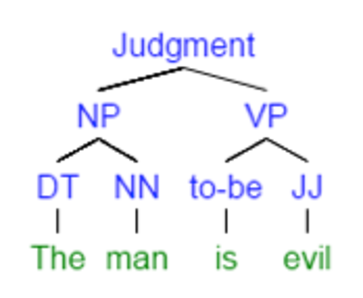
\includegraphics[width = .25\textwidth]{figs/judgment}
\caption{fig:judgment}
\label{default}
\end{center}
\end{figure}

The number of flagged sentences divided by the total number of sentences was calculated for each document. This value was averaged for each document in the bin to generate the final judgment percentage signal.

\subsection{Context Vectors}
\label{sect:cv}

\begin{equation}
V_{i}=[x_{i1},x_{i2},...,x_{iv}]
\end{equation}

\begin{equation}
c_{ij}=\sum_{k \epsilon window(w_{i})} dsm(w)
\end{equation}

\begin{equation}
semantic density(w) = \sum_{k=1}^{l-1} \frac{<c_{ik},c_{i(k+1)}>}{||c_{ik}||*||c_{i(k+1)}||}
\end{equation}


\subsection{Network Quantification}
\label{sect:network}

\section{Hyperparameter Optimization}
\label{hyper}

[Insert Text Here]

\subsection{Co-Occurrence Window}
\label{cooc window}


\subsection{Context Window}
\label{sect:context window}


\subsection{Keyword Rank Window}
\label{sect:keyword}


\subsection{Network Adjacency Angle}
\label{sect:angle}

\section{Results}
\label{results}

% acc(bin, model) = \{1, |\hat{y}-y|\}

\begin{equation}
acc(bin, model) = 
\begin{cases} 
1, & \text{if } |\hat{y}-y| \leq 1 \\
0, & \text{otherwise}
\end{cases}
\end{equation}

\begin{equation}
acc(model) = \frac{1}{|bins|} \sum_{bin  \epsilon  bins} acc(bin, model)
\end{equation}


[Insert Text Here]

\section{Conclusions}
\label{conclusions}

\section*{Acknowledgements}

The acknowledgements should go immediately before the references.  Do
not number the acknowledgements section. Do not include this section
when submitting your paper for review.


\bibliographystyle{acl}
\bibliography{coling2016}

\begin{thebibliography}{}

\bibitem[\protect\citename{Barsalou}1993]{Barsalou1993}
L.~Barsalou.
\newblock 1993.
\newblock Flexibility, structure, and linguistic vagary in concepts:
  Manifestations of a compositional system of perceptual symbols.
\newblock {\em Theories of memory}, 1:29--31.

\bibitem[\protect\citename{Blei \bgroup et al.\egroup }2003]{Blei2003}
David~M Blei, Andrew~Y Ng, and Michael~I Jordan.
\newblock 2003.
\newblock Latent dirichlet allocation.
\newblock {\em Journal of machine Learning research}, 3(Jan):993--1022.

\bibitem[\protect\citename{Boussidan and Ploux}2011]{Boussidan2011}
Armelle Boussidan and Sabine Ploux.
\newblock 2011.
\newblock Using topic salience and connotational drifts to detect candidates to
  semantic change.
\newblock In {\em Proceedings of the Ninth International Conference on
  Computational Semantics}, pages 315--319. Association for Computational
  Linguistics.

\bibitem[\protect\citename{Bullinaria and Levy}2007]{Bullinaria2007}
J.~Bullinaria and J.~Levy.
\newblock 2007.
\newblock Extracting semantic representations from word co-occurrence
  statistics: A computational study.
\newblock {\em Behavior research methods}, 39(3):510--526.

\bibitem[\protect\citename{Cook and Stevenson}2010]{Cook2010}
Paul Cook and Suzanne Stevenson.
\newblock 2010.
\newblock Automatically identifying changes in the semantic orientation of
  words.
\newblock In {\em LREC}.

\bibitem[\protect\citename{Csardi and Nepusz}2006]{Csardi2006}
Gabor Csardi and Tamas Nepusz.
\newblock 2006.
\newblock The igraph software package for complex network research.
\newblock {\em InterJournal, Complex Systems}, 1695(5):1--9.

\bibitem[\protect\citename{Estrada and Rodriguez-Velazquez}2005]{Estrada2005}
Ernesto Estrada and Juan~A Rodriguez-Velazquez.
\newblock 2005.
\newblock Subgraph centrality in complex networks.
\newblock {\em Physical Review E}, 71(5):056103.

\bibitem[\protect\citename{Evert}2014]{Evert2014}
Stefan Evert.
\newblock 2014.
\newblock Distributional semantics in r with the wordspace package.
\newblock In {\em COLING (Demos)}, pages 110--114.

\bibitem[\protect\citename{Feinerer and Hornik}2013]{Feinerer2013}
Ingo Feinerer and K~Hornik.
\newblock 2013.
\newblock tm: Text mining package. r package version 0.5-9.1.

\bibitem[\protect\citename{Hacker \bgroup et al.\egroup }2013]{Hacker2013}
K.~Hacker, D.~Boje, V.~Nisbett, A.~Abdelali, and N.~Henry.
\newblock 2013.
\newblock Interpreting iranian leaders' conflict framing by combining latent
  semantic analysis and pragmatist storytelling theory.
\newblock In {\em Political Communication Division of the National
  Communication Association annual conference}.

\bibitem[\protect\citename{Hearst}1992]{Hearst1992}
M.~Hearst.
\newblock 1992.
\newblock Automatic acquisition of hyponyms from large text corpora.
\newblock In {\em Proc. 14th Conf. Computational linguistics}, volume~2, pages
  539--545.

\bibitem[\protect\citename{Hornik and Gr{\"u}n}2011]{Hornik2011}
Kurt Hornik and Bettina Gr{\"u}n.
\newblock 2011.
\newblock topicmodels: An r package for fitting topic models.
\newblock {\em Journal of Statistical Software}, 40(13):1--30.

\bibitem[\protect\citename{Kozima}1993]{Kozima1993}
H.~Kozima.
\newblock 1993.
\newblock Text segmentation based on similarity between words.
\newblock In {\em Proc. 31st Annual Meeting Association Computational
  Linguistics}, pages 286--288.

\bibitem[\protect\citename{Lin}1998]{Lin1998}
D.~Lin.
\newblock 1998.
\newblock Automatic retrieval and clustering of similar words.
\newblock In {\em Proc. 17th Int. Conf. Computational linguistics}, volume~2,
  pages 768--774.

\bibitem[\protect\citename{Liu}2013]{Liu2013}
Bing Liu.
\newblock 2013.
\newblock A list of positive and negative opinion words or sentiment words for
  english.
\newblock {\em l{\'\i}nea]. Disponible en: http://www. cs. uic. edu/\~{}
  liub/.[{\'U}ltimo acceso: Junio 2015]}.

\bibitem[\protect\citename{Richardson}2015]{Richardson2015}
Leonard Richardson.
\newblock 2015.
\newblock Beautiful soup documentation.

\bibitem[\protect\citename{Sagi \bgroup et al.\egroup }2009]{Sagi2009}
Eyal Sagi, Stefan Kaufmann, and Brady Clark.
\newblock 2009.
\newblock Semantic density analysis: Comparing word meaning across time and
  phonetic space.
\newblock In {\em Proceedings of the Workshop on Geometrical Models of Natural
  Language Semantics}, pages 104--111. Association for Computational
  Linguistics.

\bibitem[\protect\citename{Searcey and Santora}2015]{Searcey2015}
D.~Searcey and M.~Santora.
\newblock 2015.
\newblock Boko haram tops isis in ranking terror groups.
\newblock {\em New York Times}, page~A6, November.

\bibitem[\protect\citename{Yang \bgroup et al.\egroup }2010]{Yang2010}
M.~Yang, S.~Wong, and J.~Coid.
\newblock 2010.
\newblock The efficacy of violence prediction: a meta-analytic comparison of
  nine risk assessment tools.
\newblock {\em Psychological bulletin}, 136(5):740.

\end{thebibliography}

\end{document}
